\documentclass{article}
\usepackage{graphicx}
\usepackage{listings}
\usepackage{color}
\usepackage{amsmath}
\usepackage{amsfonts}
\usepackage{bm}
\usepackage[utf8]{inputenc}

\title{Modelli dinamici Pt.2\\
	Corso di LSMC, a.a. 2017-2018}
\author{Davide Gori\\
	550282}


\definecolor{backcolour}{rgb}{0.95,0.95,0.92}
\definecolor{gray}{rgb}{0.5,0.5,0.5}
\lstset{basicstyle=\ttfamily\small,
	columns=fullflexible,
	numbers=left,
	numberstyle=\tiny\ttfamily\color{gray},
	backgroundcolor=\color{backcolour},
	tabsize=4,
	language=Octave
}


\begin{document}
	\maketitle
	\section{Prima sperimentazione: moto di un punto vincolato}
	Il moto di un punto $z(x) = [z_1(x), z_2(x), z_3(x)]^T$ di massa $m$ soggetto alla forza di	gravità $F=[0, 0, -gm]^T$ è vincolato a muoversi sulla superficie sferica di equazione $\phi(\mathbf{z})=z_1^2+z_2^2+z_3^2-1=0$ è descritto dal seguente sistema di equazioni differenziali ordinarie:
	$$\mathbf{z}''=\frac{1}{m} \left(\mathbf{F}-\frac{m\mathbf{z'^T}H\mathbf{z'}+\nabla\phi^T\mathbf{F}}{\left|\nabla\phi\right|^2} \nabla\phi\right), x>0$$
	Con condizioni iniziali $\mathbf{z(0)}=\mathbf{z_0}$, $\mathbf{z'(0)}=\mathbf{v_0}$.\\
	Dove abbiamo indicato con $\nabla\phi$ il gradiente di $\phi$ e con $H$ la matrice hessiana di $\phi$.\\
	Modellizzo il seguente problema come problema di Caucy con incognita $\mathbf{y}$, dove $y(1) = z(1)$, $y(2) = z(2)$, $y(3) = z(3)$, $y(4) = z'(1)$, $y(5) = z'(2)$, $y(6) = z'(3)$.\\
	Risolvo il problema con le seguenti condizioni iniziali: $y_0=[0, 1, 0, 0.8, 0, 1.2]$, nell'intervallo di integrazione $[0, 10]$ e $m=1$.\\
	Applicando il metodo di Eulero esplicito (con $h = 0.0025$ e $h = 0.00025$), il metodo di Runge-Kutta classico (con $h = 0.005$ e $h = 0.0005$) e le funzioni predefinite {\tt ode23} e {\tt ode45}, quest'ultima con valori di {\tt RelTot} pari a $10^{-3}$ (valore di default) e $10^{-6}$.\\
	La bontà della soluzione si può stimare calcolando il massimo valore di $r=\left|y_1^2+y_2^2+y_3^2-1\right|$, visto che la soluzione non approssimata soddisfa sempre $r=0$.
	\subsection{Il codice}
	Questo è lo script che realizza lasperimentazione:
	\lstinputlisting{LabSper_6_1.m}
	\subsection{Risultati}
	Riportiamo i grafici in output.\\
	Dove il massimo del parametro $r$ vale, in ordine:
	\begin{itemize}
		\item $r = 0.44791$.
		\item $r = 0.043485$.
		\item $r = 4.7988e-06$.
		\item $r = 4.8007e-10$.
		\item $r = 0.0092088$.
		\item $r = 0.55712$.
		\item $r = 1.0655e-04$.
	\end{itemize}
	\begin{figure}[htp!]
		\centering 
		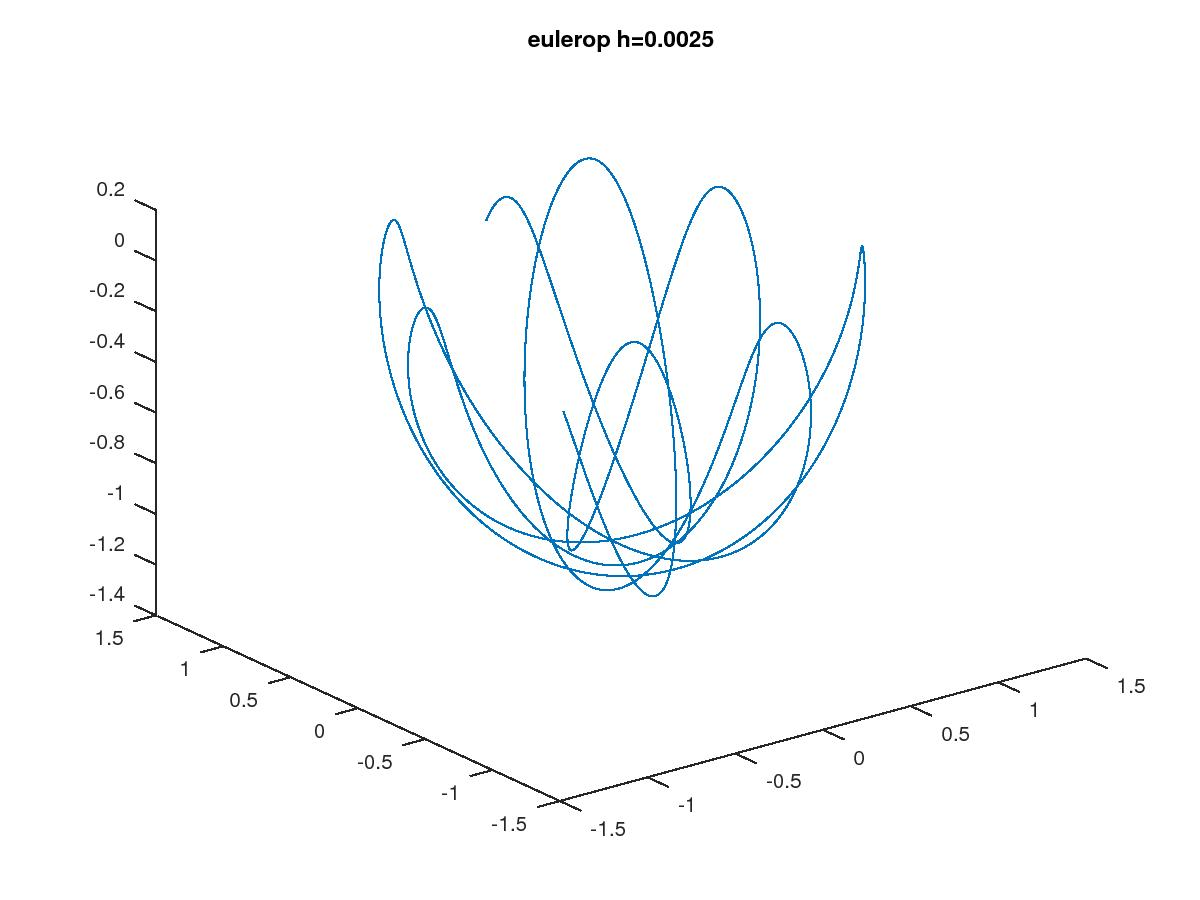
\includegraphics[width=\textwidth]{6_1_1.jpeg}
	\end{figure}
	\begin{figure}[htp!]
		\centering 
		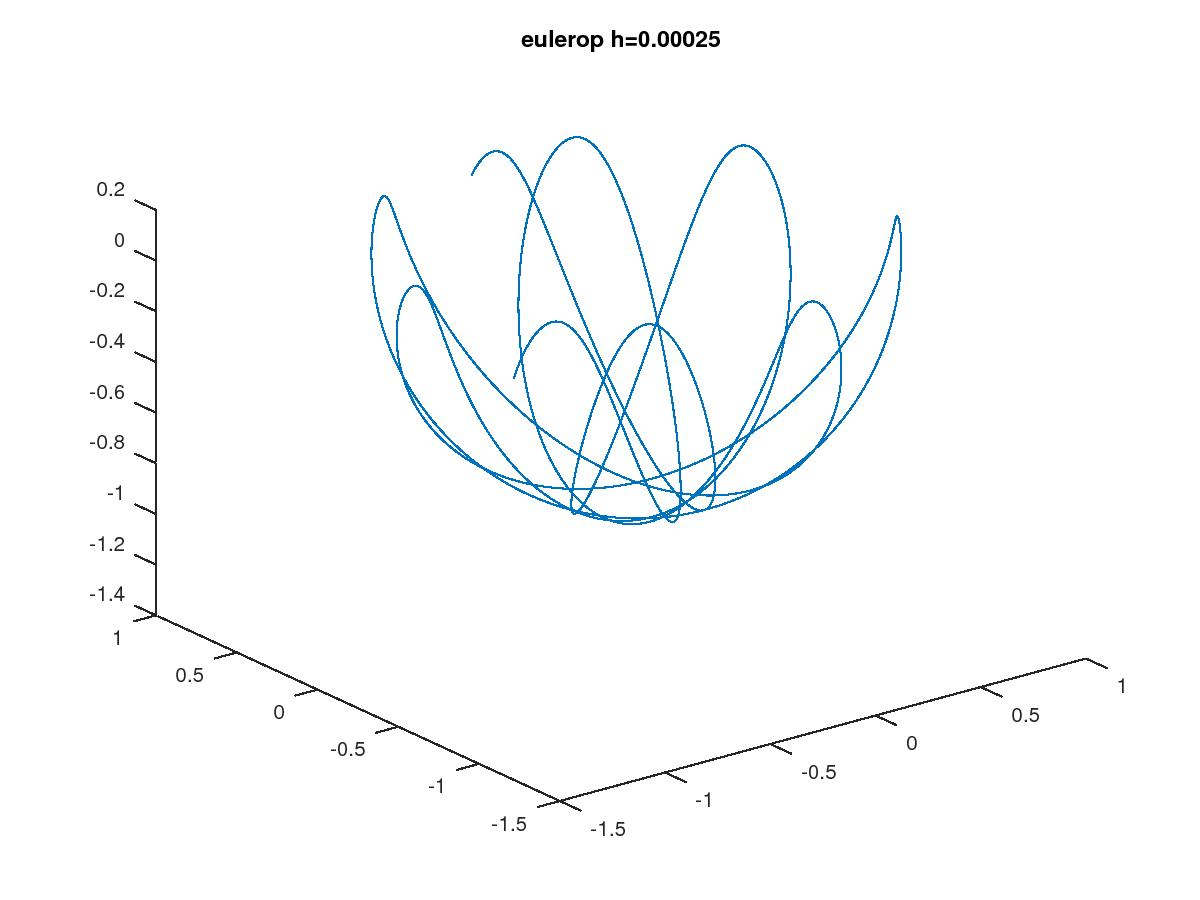
\includegraphics[width=\textwidth]{6_1_2.jpeg}
	\end{figure}
	\begin{figure}[htp!]
		\centering 
		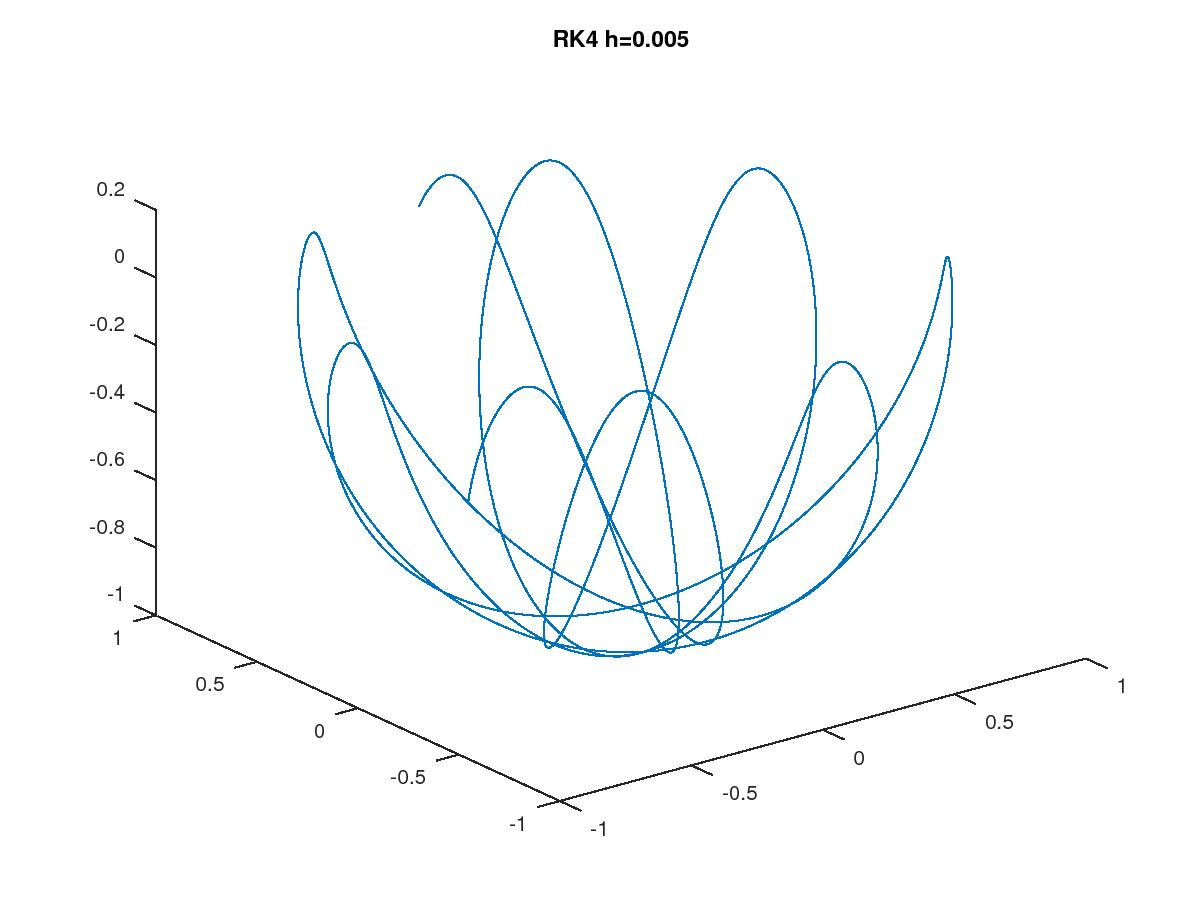
\includegraphics[width=\textwidth]{6_1_3.jpeg}
	\end{figure}
	\begin{figure}[htp!]
		\centering 
		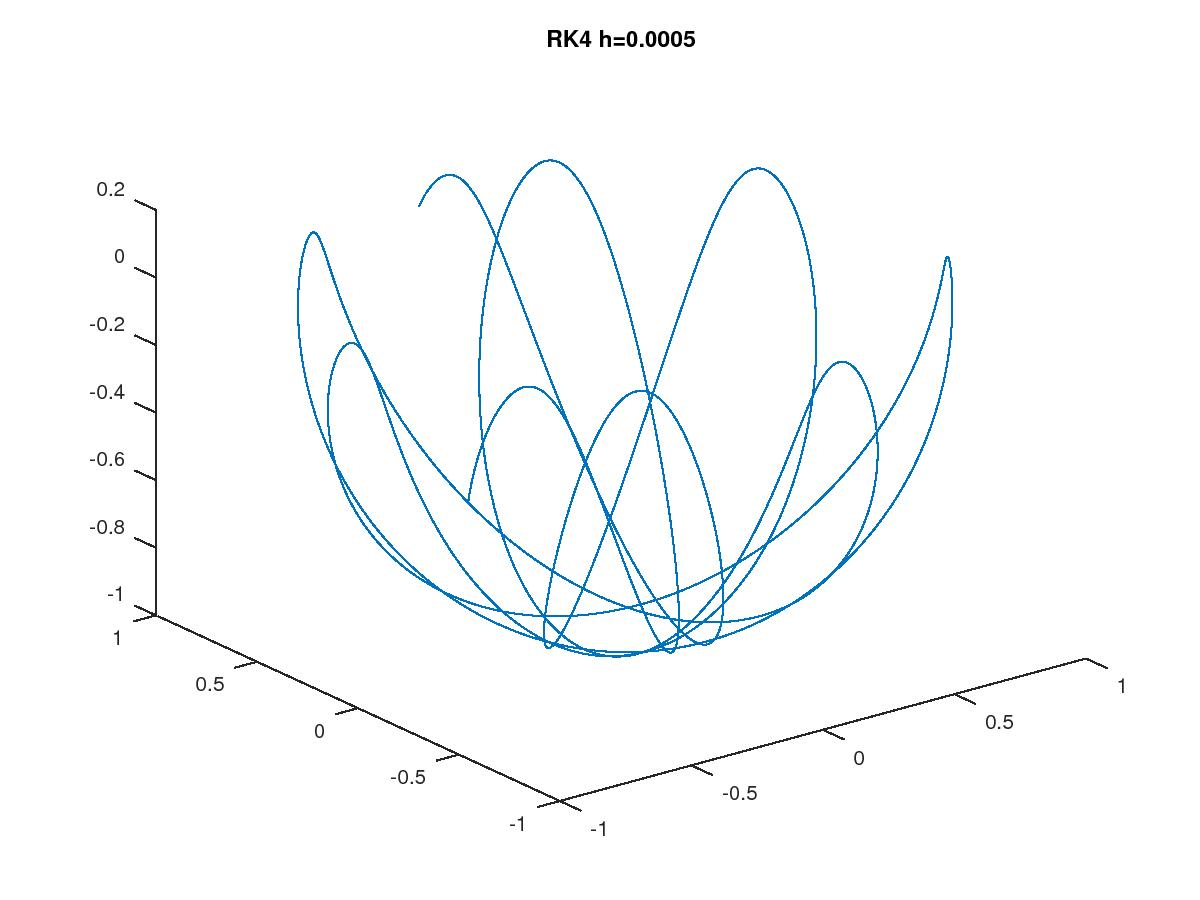
\includegraphics[width=\textwidth]{6_1_4.jpeg}
	\end{figure}
	\begin{figure}[htp!]
		\centering 
		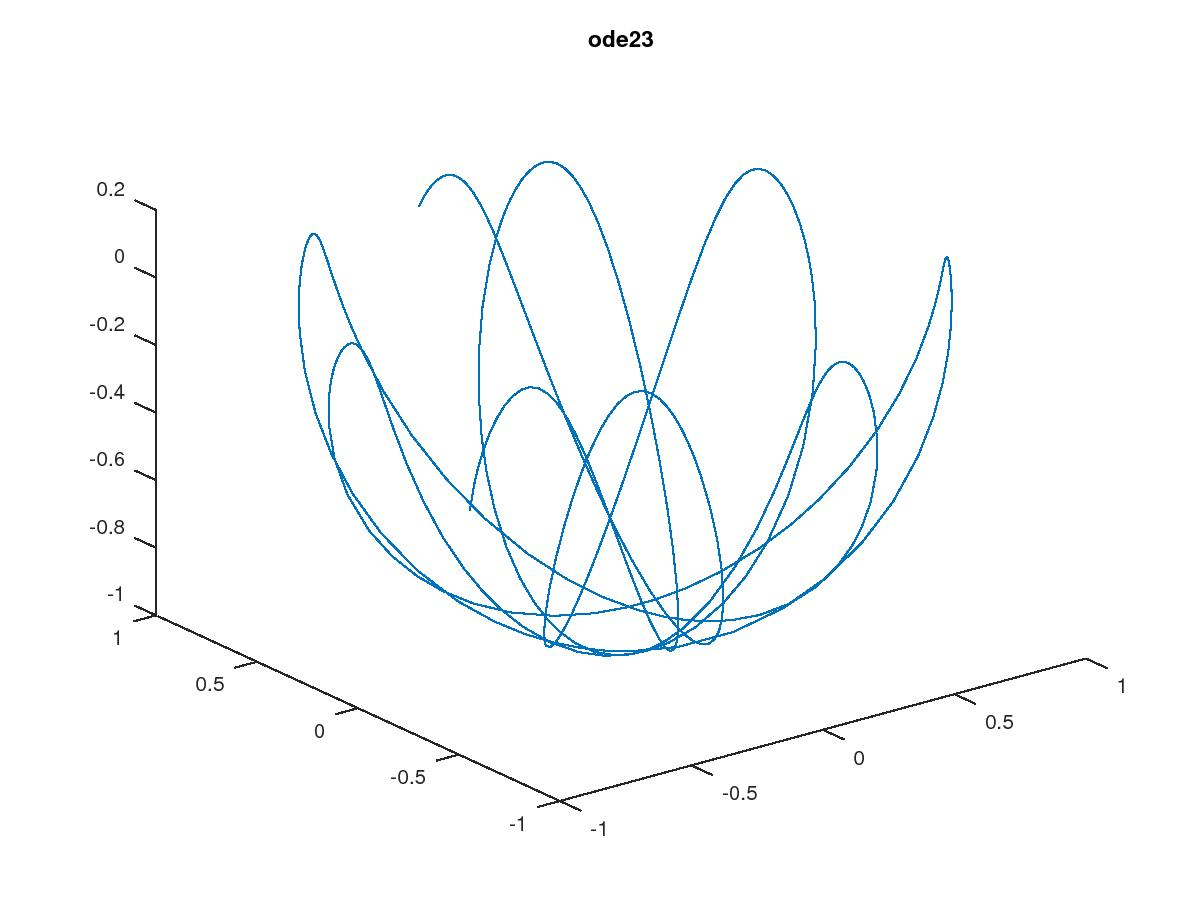
\includegraphics[width=\textwidth]{6_1_5.jpeg}
	\end{figure}
	\begin{figure}[htp!]
		\centering 
		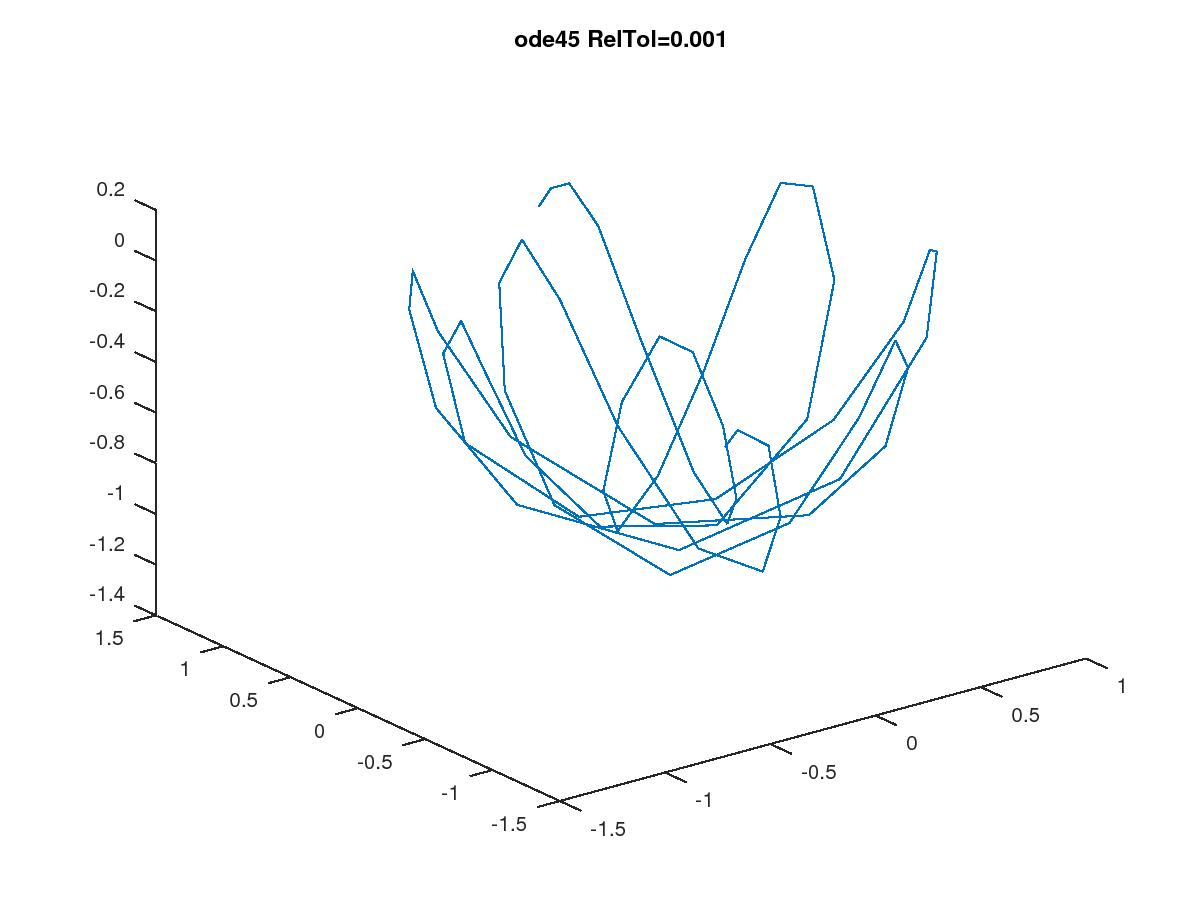
\includegraphics[width=\textwidth]{6_1_6.jpeg}
	\end{figure}
	\begin{figure}[htp!]
		\centering 
		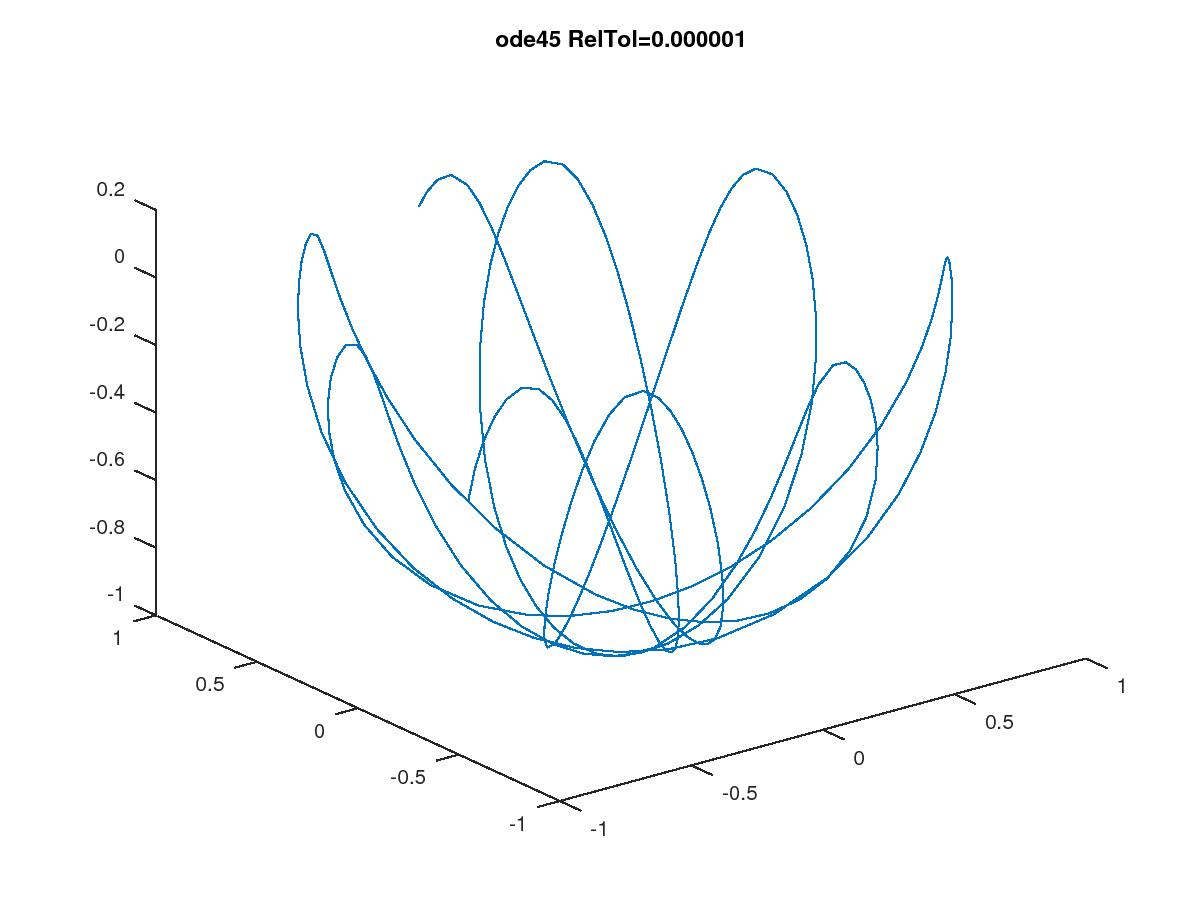
\includegraphics[width=\textwidth]{6_1_7.jpeg}
	\end{figure}
	\newpage
	\section{Seconda sperimentazione: modello di Lorentz}
	Calcolo la soluzione numerica del modello di Lorenz nel caso $\sigma = 10$, $r = 28$, $b = \frac{8}{3}$ a partire dalle seguenti condizioni iniziali:\\
	$y_1(0) = 10$, $y_2(0) = 0$, $y_3(0) = 20$.\\
	$y_1(0) = 11$, $y_2(0) = 0$, $y_3(0) = 20$.\\
	Per un tempo $x_max$ adeguato. Realizzando separatamente i grafici di $(x, y_1)$, $(x, y_2)$,
	$(x, y_3)$, $(y_1, y_2, y_3)$.
	\subsection{Il codice}
	Questo è lo script che realizza la sperimentazione:
	\lstinputlisting{LabSper_6_2.m}
	
	\subsection{Risultati}
	Riportiamo i grafici in output.\\
	Dove i dati relativi al primo caso sono in blu e in rosso quelli relativi al secondo.\\
	Si puà osservare che, pur essendo i dati iniziali molto vicini, il comportamento della soluzione per tempi grandi risulta completamente diverso nei
	due casi.\\
	\begin{figure}[htp!]
		\centering 
		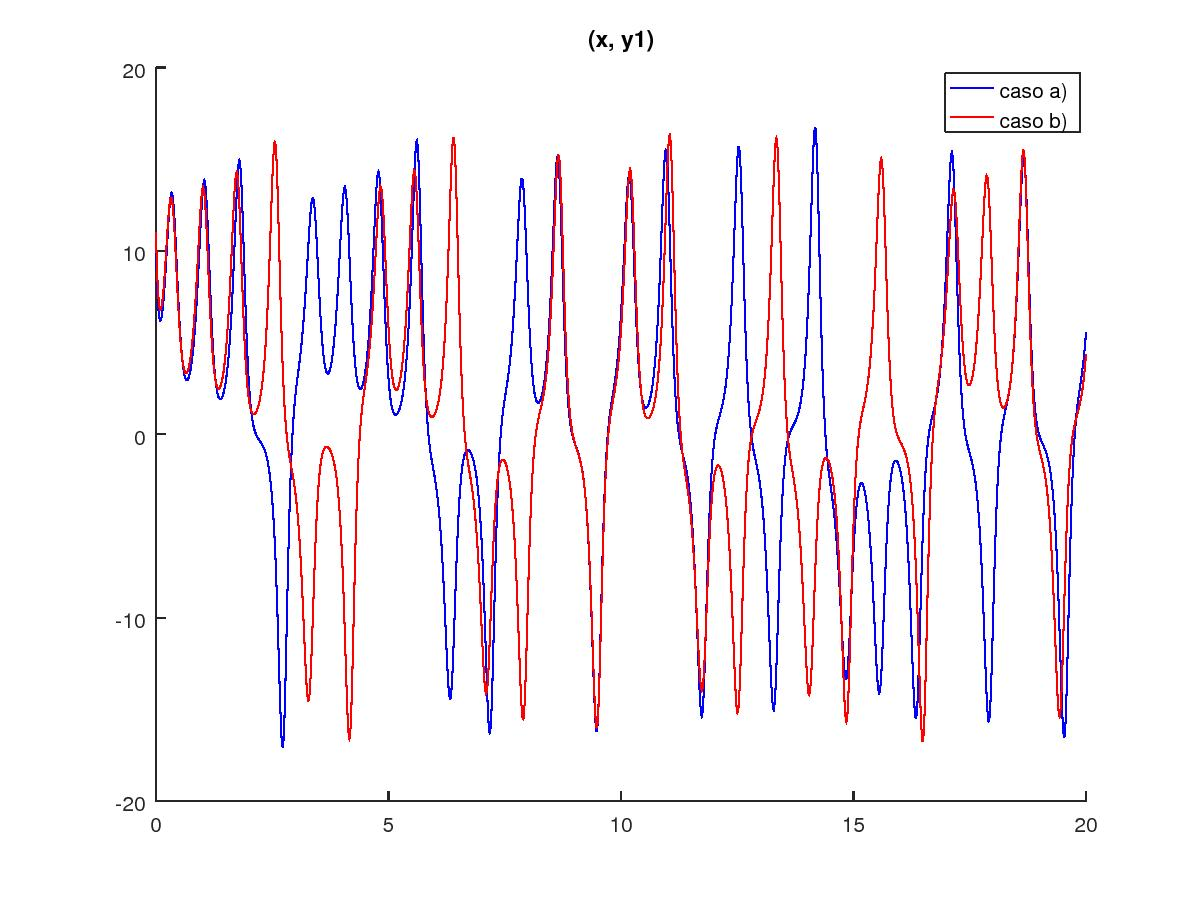
\includegraphics[width=\textwidth]{6_2_1.jpeg}
	\end{figure}
	\begin{figure}[htp!]
	\centering 
	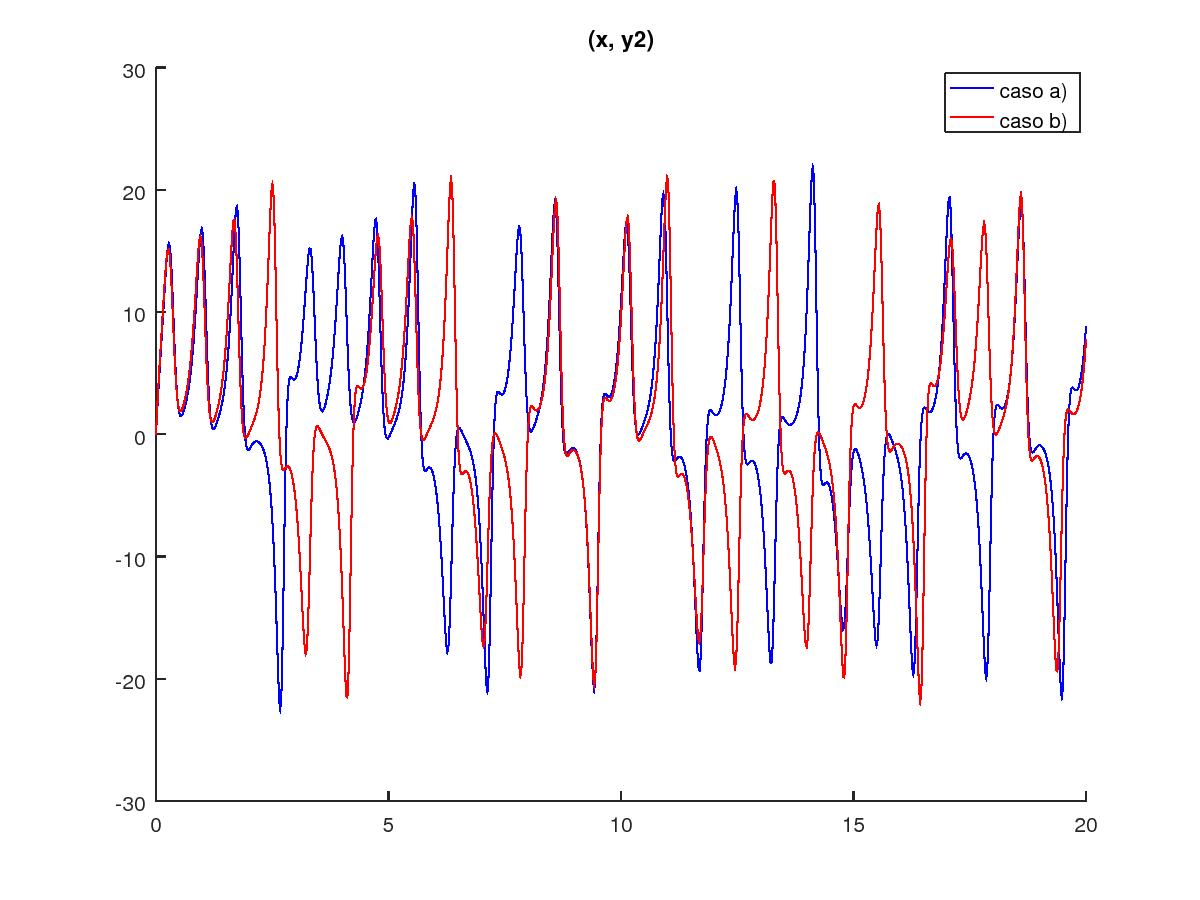
\includegraphics[width=\textwidth]{6_2_2.jpeg}
	\end{figure}
	\begin{figure}[htp!]
	\centering 
	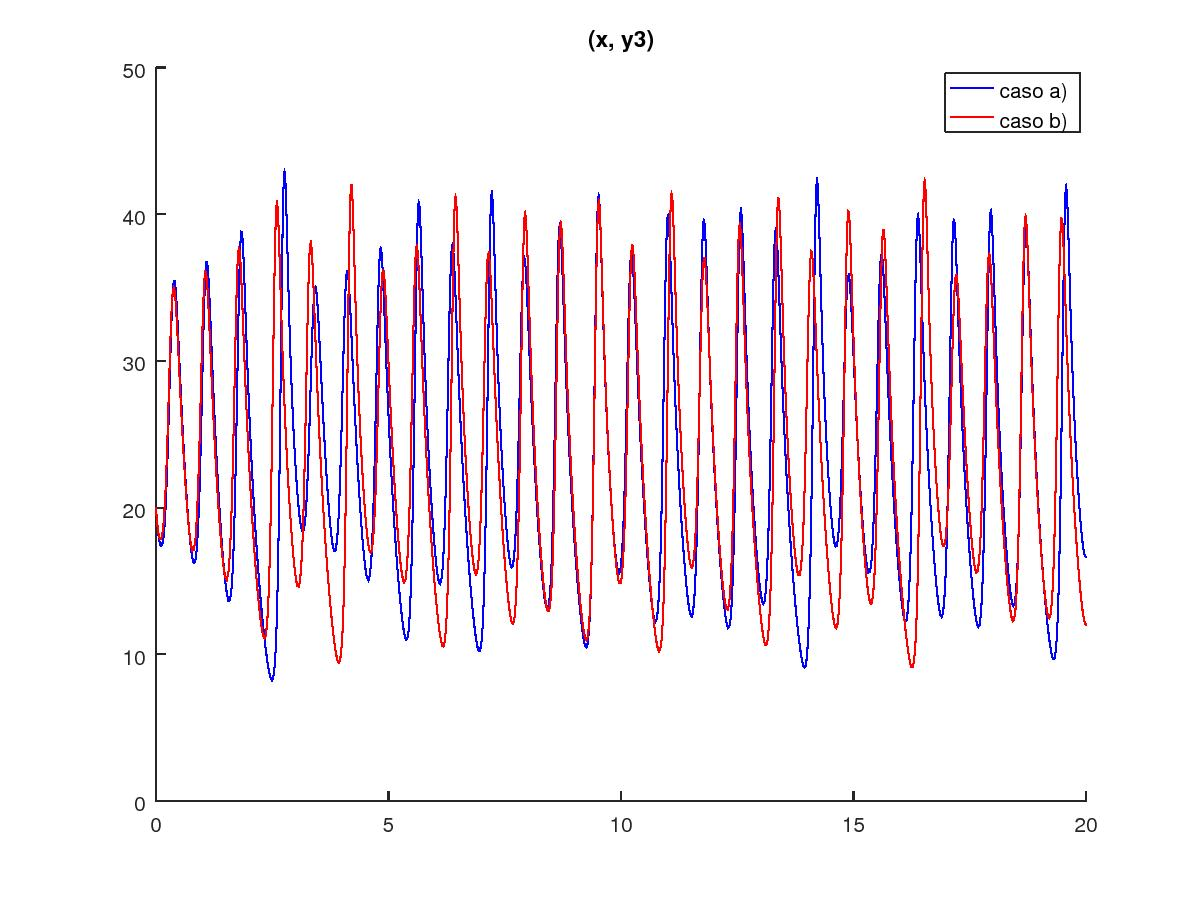
\includegraphics[width=\textwidth]{6_2_3.jpeg}
	\end{figure}
	\begin{figure}[htp!]
	\centering 
	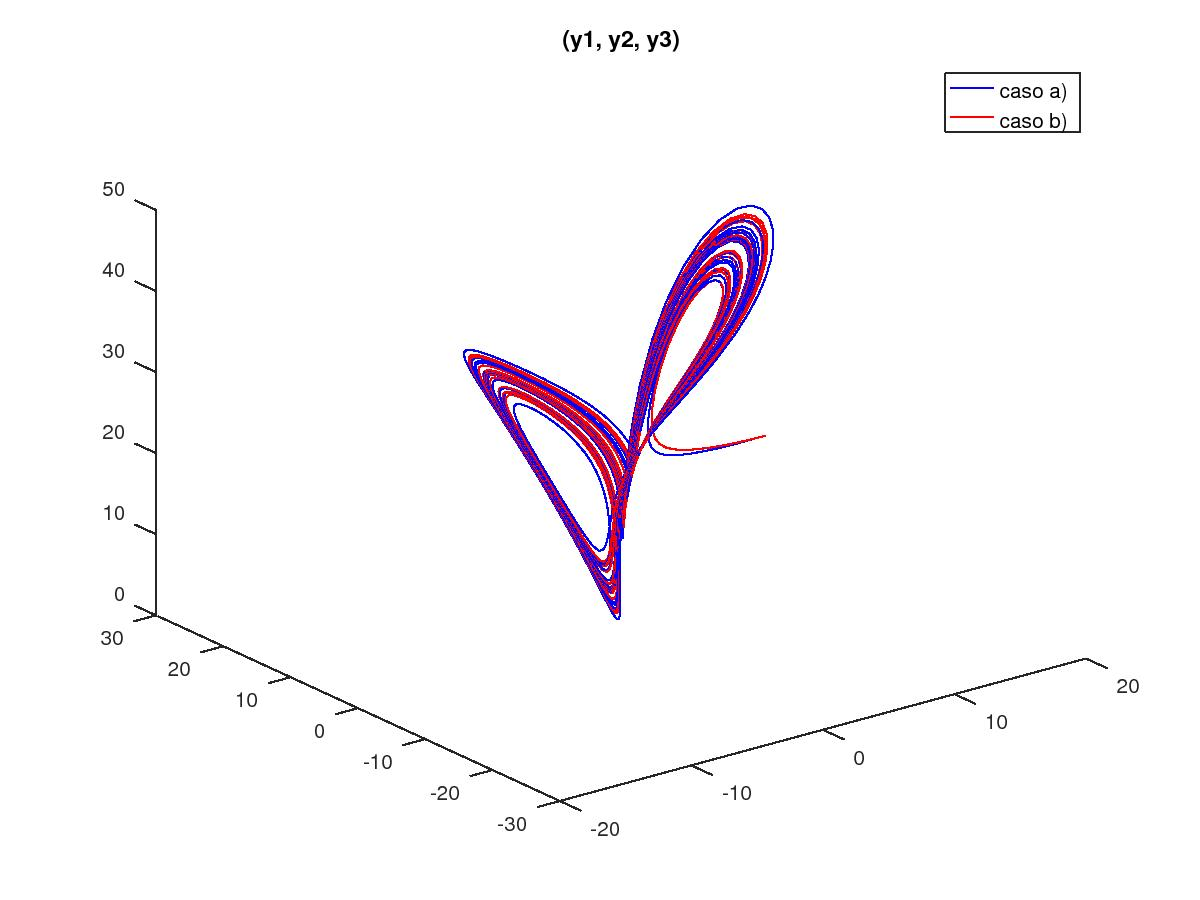
\includegraphics[width=\textwidth]{6_2_4.jpeg}
	\end{figure}
	Notiamo che $y_1$ e $y_2$ si hanno comportamenti diversi per i due dati iniziali, mentre $y_3$ ha un comportamento più simile nelle due sperimentazioni.
	\newpage
	\section{Terza sperimentazione: equazione di Van der Pol}
	L'equazione di Van der Pol governa l'intensità di corrente $y(x)$ in un circuito oscillante a triodo e viene utilizzata nello studio di circuiti che contengono valvole termoioniche, i cosiddetti tubi a vuoto, come il magnetron nei forni a microonde. L’equazione ha la forma seguente:
	$$y''=\mu(1-y^2)y'-y$$
	dove $\mu$ indica l'intensità dello smorzamento non lineare. Per valori di $\mu$ piccoli, $y$ ha un comportamento transitorio oscillante che evolve in un comportamento a regime di
	forma simile ad una sinusoide. Invece per valori di $\mu$ grandi il comportamento di $y$ presenta rapide transizioni intercalate da periodi più tranquilli.\\
	Vogliamo studiare questo fenomeno.
	\subsection{L'implementazione}
	Risolveremo numericamente questa equazione sull'intervallo $[0, 100]$ applicando {\tt ode45} oppure {\tt eulero} con le condizioni iniziali $y(0) = 1$ e $y'(0) = 1$ per i casi $\mu = 0.1, 1, 10, 100$.\\
	Per ciascun caso disegneremo la traiettoria di $y$ in funzione di $x$.
	\subsection{Il codice}
	Questo è lo script che realizza la sperimentazione:
	\lstinputlisting{LabSper_6_3.m}
	
	\subsection{Risultati}
	Riportiamo i grafici in output.\\
	Il secondo grafico di ogni coppia rappresenta la distribuzione dei nodi nel caso {\tt ode45}, la non linearità del grafico è sintomo di "difficoltà" numerica.\\
	\begin{figure}[htp!]
		\centering 
		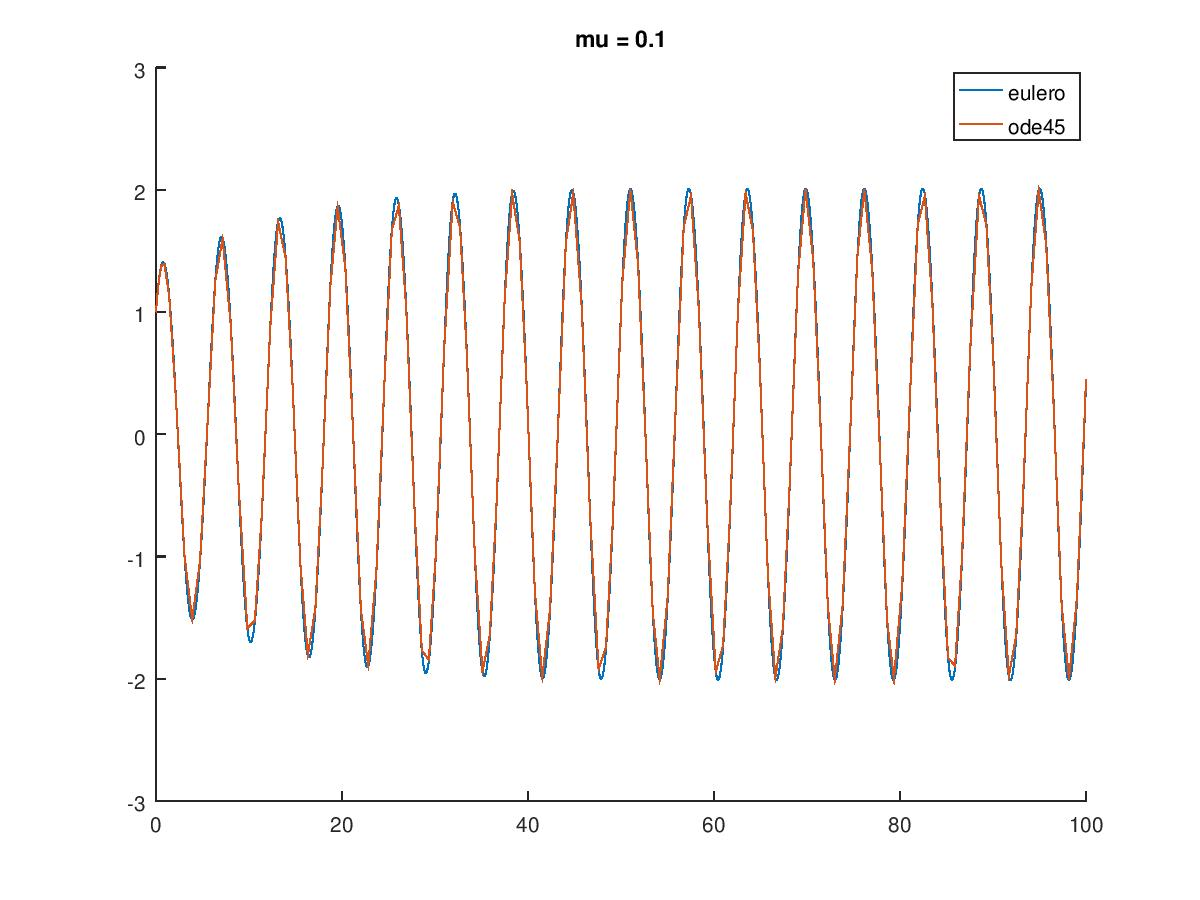
\includegraphics[width=\textwidth]{6_3_1.jpeg}
	\end{figure}
	\begin{figure}[htp!]
		\centering 
		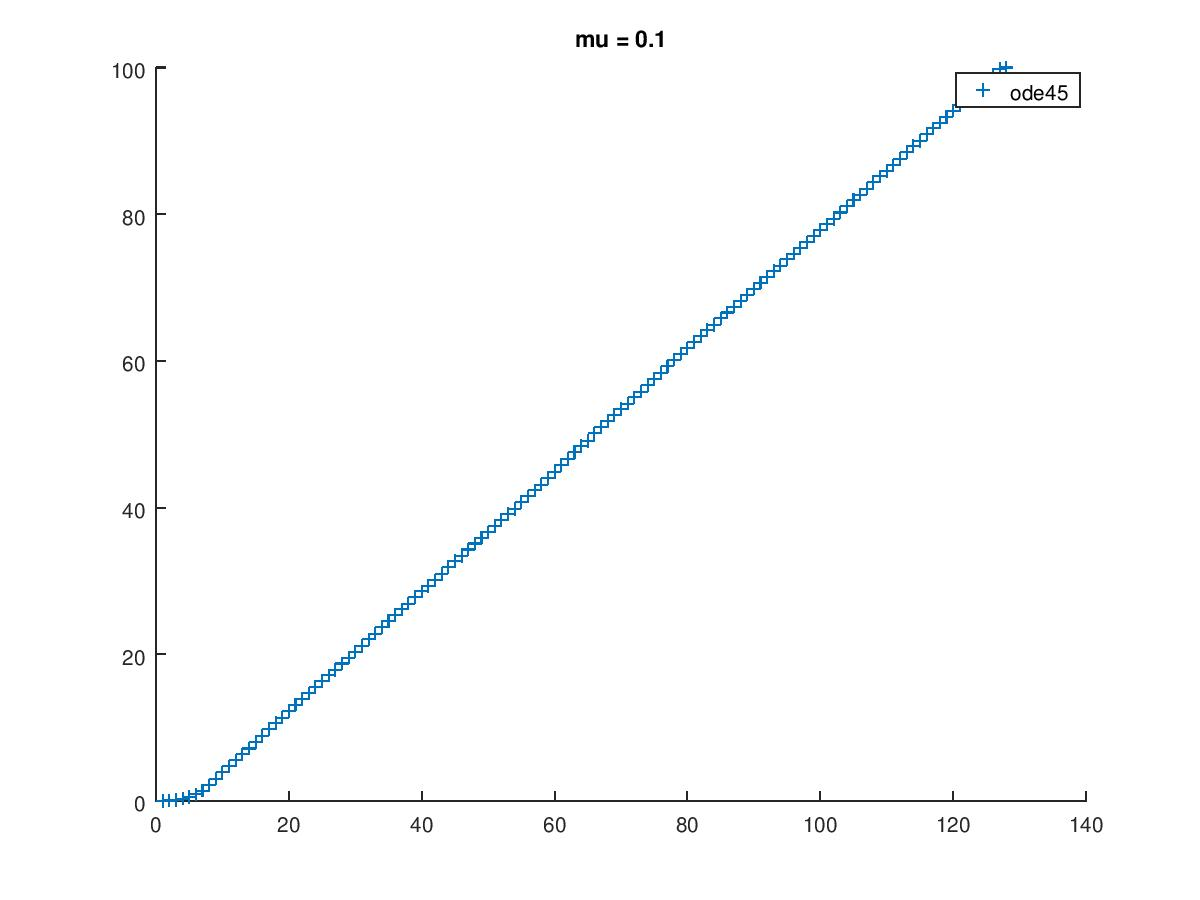
\includegraphics[width=\textwidth]{6_3_1_a.jpeg}
	\end{figure}
	\begin{figure}[htp!]
		\centering 
		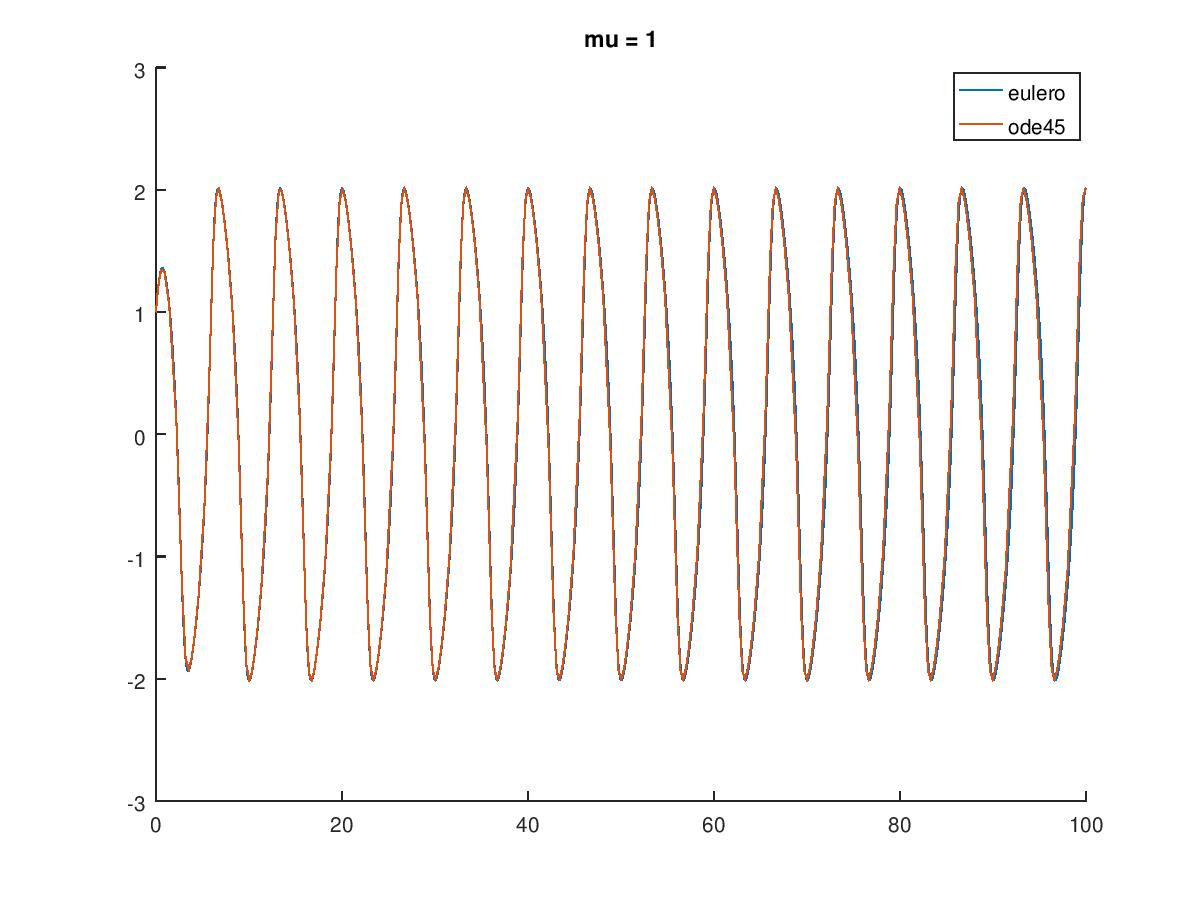
\includegraphics[width=\textwidth]{6_3_2.jpeg}
	\end{figure}
	\begin{figure}[htp!]
		\centering 
		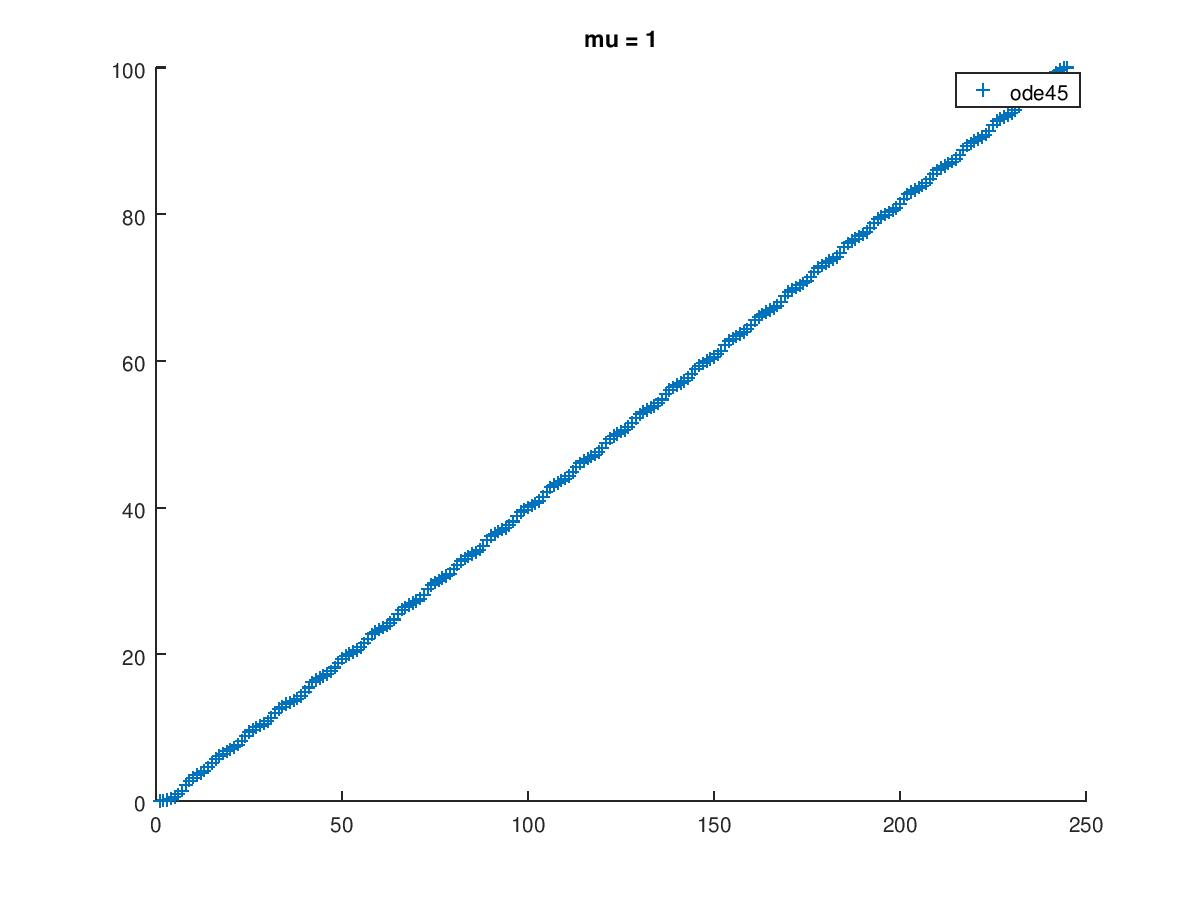
\includegraphics[width=\textwidth]{6_3_2_a.jpeg}
	\end{figure}
	\begin{figure}[htp!]
		\centering 
		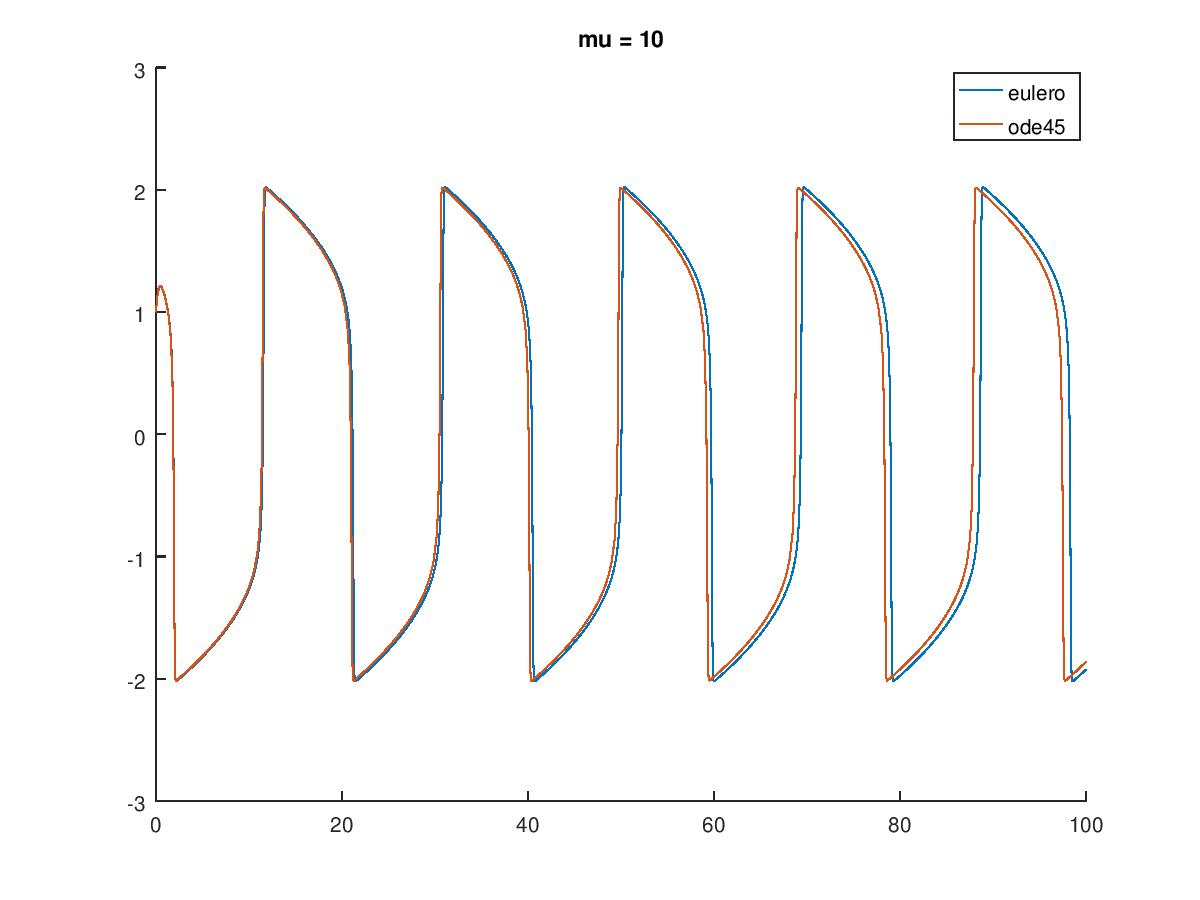
\includegraphics[width=\textwidth]{6_3_3.jpeg}
	\end{figure}
	\begin{figure}[htp!]
		\centering 
		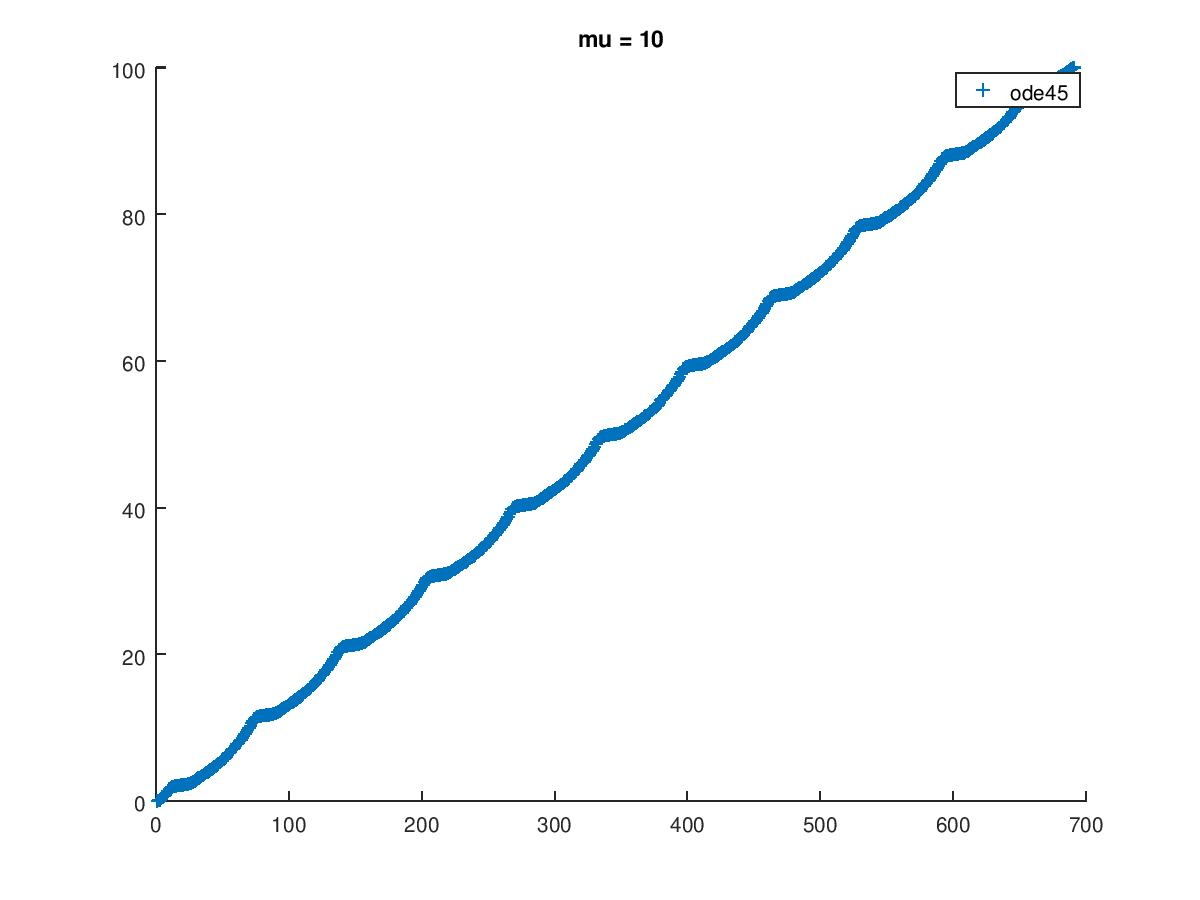
\includegraphics[width=\textwidth]{6_3_3_a.jpeg}
	\end{figure}
	\begin{figure}[htp!]
		\centering 
		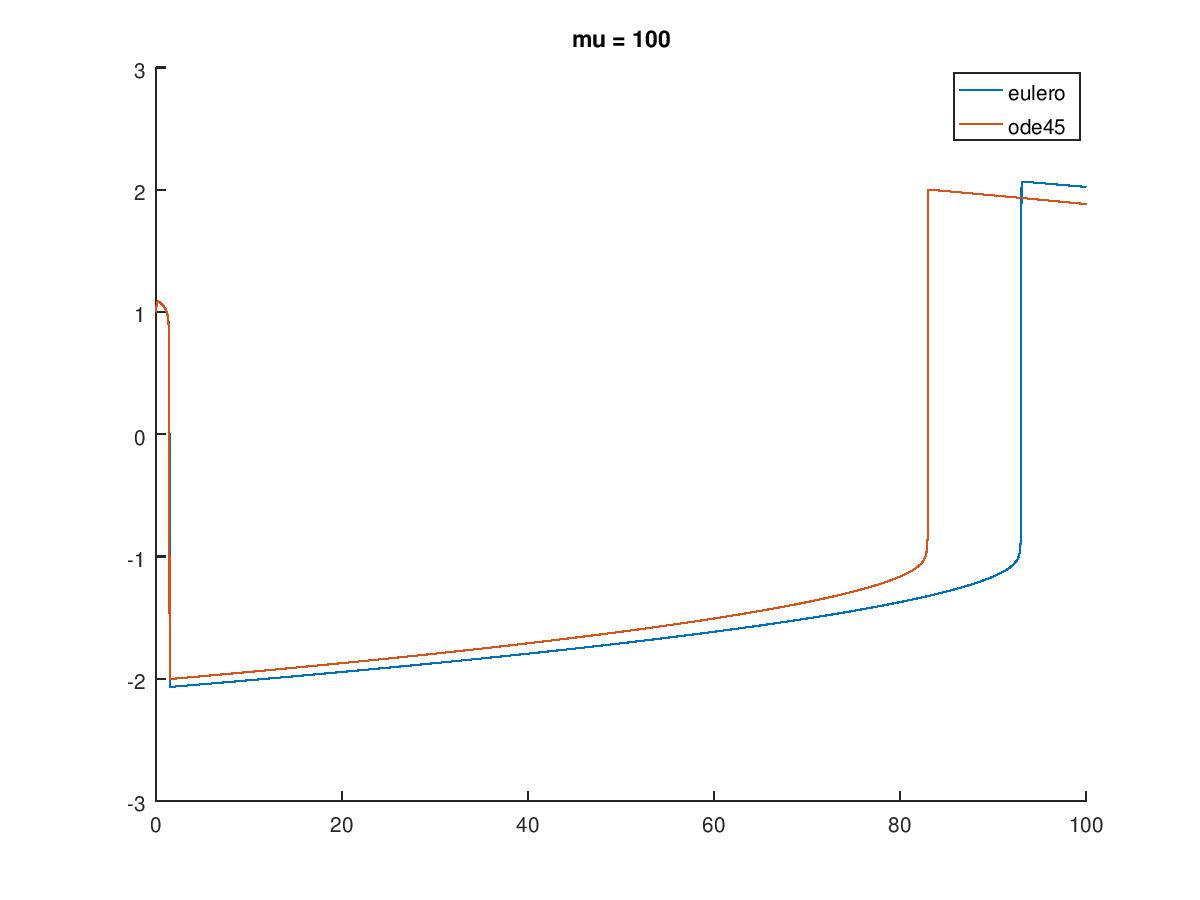
\includegraphics[width=\textwidth]{6_3_4.jpeg}
	\end{figure}
	\begin{figure}[htp!]
		\centering 
		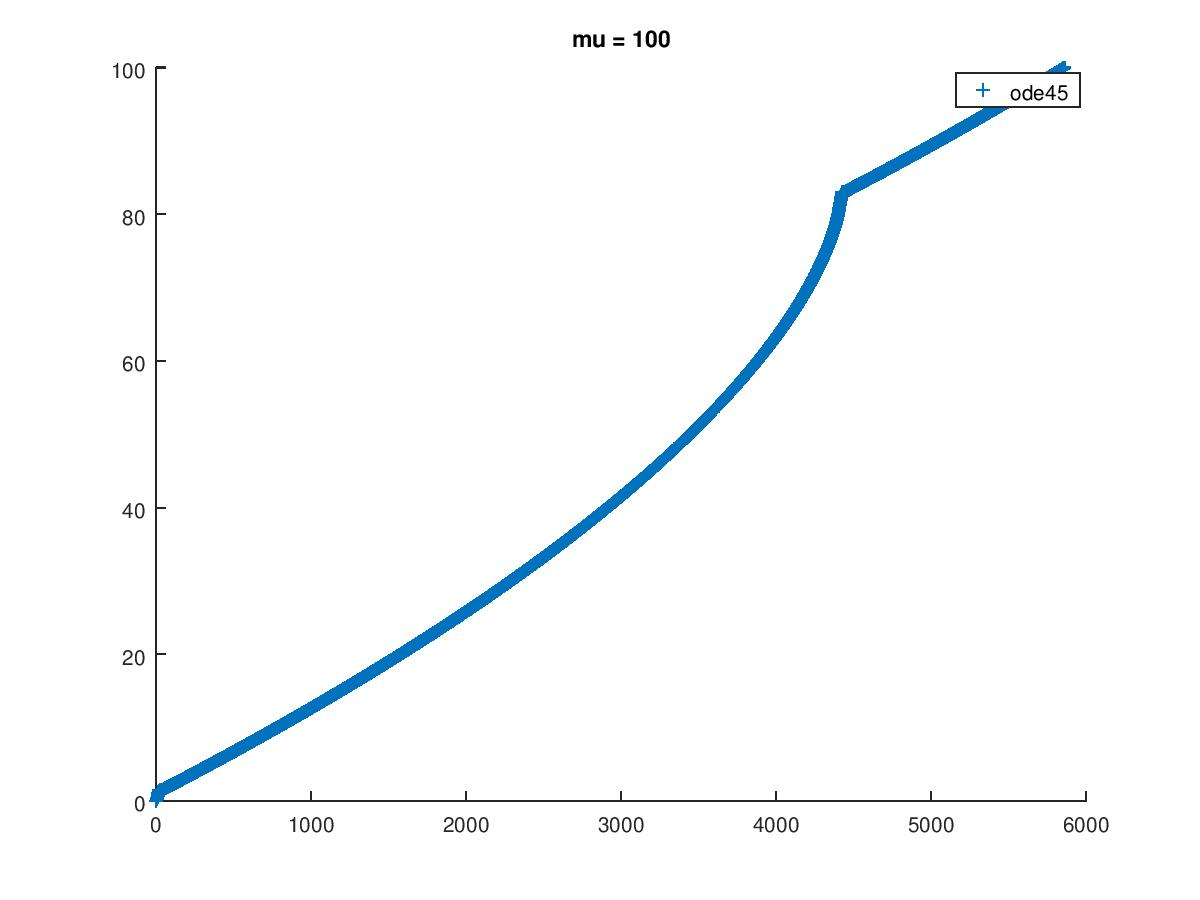
\includegraphics[width=\textwidth]{6_3_4_a.jpeg}
	\end{figure}
\end{document}